%\documentclass[letterpaper,12pt]{article}
\documentclass{mcp}

\usepackage{graphics}

\usepackage{geometry}
%\usepackage{amsmath}
%\usepackage{amsfonts}
\usepackage{amssymb}
\usepackage{bm}
\usepackage{algorithmic}
\usepackage{algorithm}
\usepackage{rotating}
\usepackage{color}
\usepackage{tikz}
\usetikzlibrary{shapes,arrows,backgrounds,calc,positioning,fit,petri,plotmarks}
\usepackage{multirow}
\usepackage{graphicx}
\usepackage{caption}
\usepackage{subcaption}
\usepackage{url}
\usepackage{booktabs}
\usepackage{enumitem}
\usepackage{authblk}
\usepackage{xr}
\usepackage{hyperref}
\externaldocument[main-]{../main/MSstatsPTM_Main}

\usepackage[backend=biber,sorting=none]{biblatex}
\bibliography{ptm_ref}

\def\todo#1{{\color{red}[TODO: #1]}}


\DeclareCaptionFormat{subfig}{\figurename~#1#2#3}
\DeclareCaptionSubType*{figure}
\captionsetup[subfigure]{format=subfig,labelsep=colon,labelformat=simple}


%\usepackage{caption} 
%\captionsetup[table]{skip=10pt}
\captionsetup{belowskip=12pt,aboveskip=4pt}

% strikkeout \sout
\usepackage[normalem]{ulem}


\usepackage{fullpage}
\usepackage{amsfonts,amsthm}
\usepackage{amsmath}
%\usepackage[fleqn]{amsmath}
%\usepackage{setspace}
%\usepackage{url}

%\usepackage[table,dvipsnames]{xcolor}
%\usepackage{textcomp}
%\usepackage{gensymb}

\usepackage{fancyhdr}
\pagestyle{fancy}
\lhead{\footnotesize \parbox{11cm}{Supplementary}}
\headsep = 25pt

%\usepackage{tabulary,multirow,multicol,rotating}

%% big wide hat
\usepackage{scalerel,stackengine}
\stackMath
\newcommand\reallywidehat[1]{%
\savestack{\tmpbox}{\stretchto{%
  \scaleto{%
    \scalerel*[\widthof{\ensuremath{#1}}]{\kern-.6pt\bigwedge\kern-.6pt}%
    {\rule[-\textheight/2]{1ex}{\textheight}}%WIDTH-LIMITED BIG WEDGE
  }{\textheight}% 
}{0.5ex}}%
\stackon[1pt]{#1}{\tmpbox}%
}
\parskip 1ex

\renewcommand{\thetable}{S\arabic{table}}
\renewcommand{\thefigure}{S\arabic{figure}}
%\renewcommand{\tablename}{Supplementary Table}
%\renewcommand{\figurename}{Supplementary Figure}

\def\sfigref#1{{Figure~\ref{#1}}}
\def\secref#1{Section~\ref{#1}}
\def\stabref#1{{Table~\ref{#1}}}
\def\seqref#1{Eq.~(\ref{#1})}

%\floatname{algorithm}{Procedure}
%\renewcommand{\algorithmicrequire}{\textbf{Input:}}
%\renewcommand{\algorithmicensure}{\textbf{Output:}}


\title{MSstatsPTM statistical relative quantification of post-translational modifications in global proteomics experiments\\
\textbf{Supplementary Information}
}

\author[1]{Devon~Kohler}
\author[2]{Tsung-Heng~Tsai}
\author[4]{Erik~Verschueren}
\author[1]{Ting~Huang}
\author[3]{Trent~Hinkle}
\author[3]{Lilian~Phu}
\author[3]{Meena~Choi*}
\author[1]{Olga~Vitek*}
\affil[1]{Khoury College of Computer Science, Northeastern University, Boston, MA, USA}
\affil[2]{Kent State University, Kent, OH, USA}
\affil[3]{MPL, Genentech, South San Francisco, CA, USA}
\affil[4]{ULUA BV, Arendstraat 29, 2018 Antwerp, Belgium}
\affil[*]{Corresponding Authors}

\date{}


\begin{document}
\maketitle

\newpage
\tableofcontents

%%%%%%%%%%%%%%%%%%%%%%%%%%%%%%%%%%%%%%%%%%%%%%%%%%%%%%%%%%%%%%%%
\clearpage
\section{Details of the proposed approach}
\label{sec:prop}


\begin{figure}[h!]
\makebox[\textwidth][c]{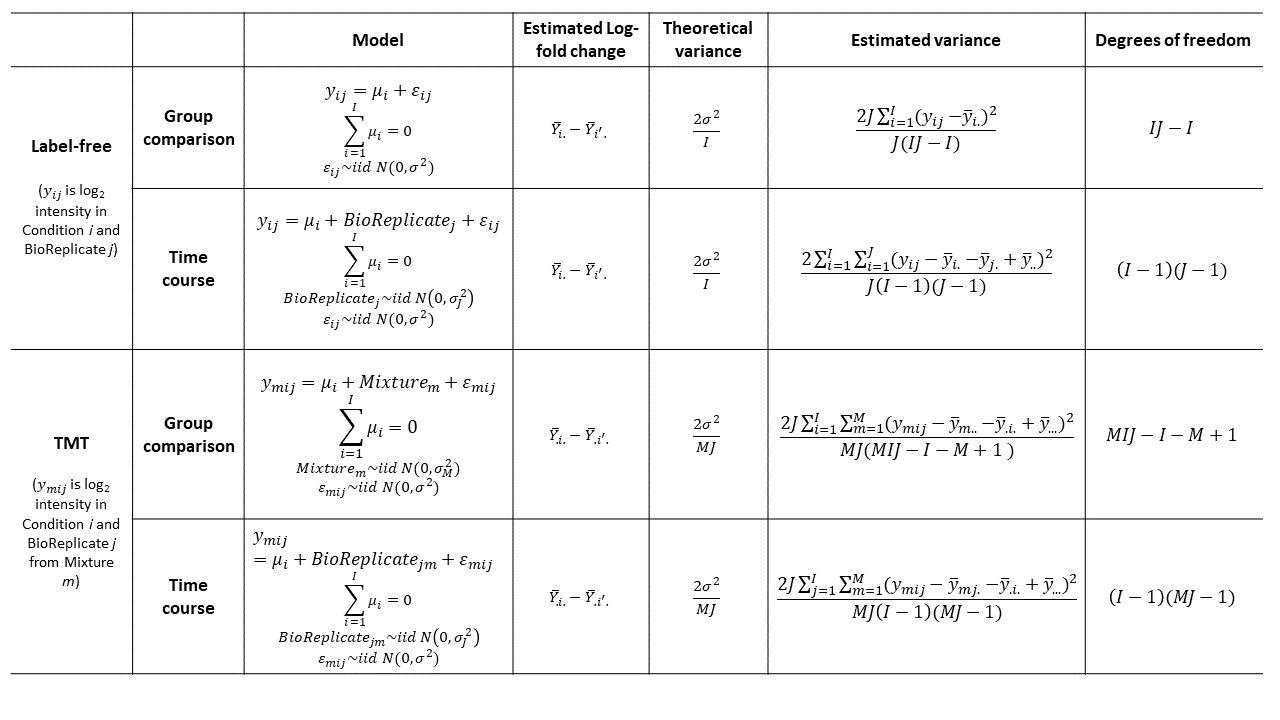
\includegraphics[width=1.2\textwidth]{sim_new/Statistical_inference}}%
\caption{Different models that are fit depending on the experimental design (group comparison and time course) and quantification workflow (label-free versus TMT). The table shows the true values of the standard errors, along with their estimates and the associated degrees of freedom. The same formulas holds when comparing changes in PTM, or hcnges in the unmodified portion of the protein. When combining the two comparisons for an adjustment, the variance must be multiplied by 2. \label{fig:statistical_inference}}
\end{figure}


%%%%%%%%%%%%%%%%%%%%%%%%%%%%%%%%%%%%%%%%%%%%%%%%%%%%%%%%%%%%%%%%
\clearpage
\section{Details on the generation of simulated datasets}
\label{sec:experiments}


%%%%%%%%%%%%%%%%%%%%%%%%%%%%%%%%%%%%%%%%%%e%%%%%%%%%%%%%%%%%%%%%%
\subsection{Dataset 1 : Computer simulation 1 - Label-free}
\label{sec:dataset1}

In the first simulation an experiment with many features per PTM and unmodified protein was created. Additionally this simulation contained no missing data.

\begin{itemize}
\item Mean of log-intensity: $25$
\item Standard deviations of log-intensities for modified and unmodified peptides: $0.2$, $0.3$
\item Difference in PTM abundance between conditions: $0$, $1.$, $2.$, $3.$
\item Difference in protein abundance between conditions: $0$, $1.$, $2.$, $3.$
\item Number of replicates: $2$, $3$, $5$, $10$
\item Number of conditions: $2$, $3$, $4$
\item Number of realizations: $1000$
\item Number of features per PTM: $10$
\item Number of features per unmodified protein: $10$
\item Missing data: no missing value
\end{itemize}

\subsection{Dataset 2 : Computer simulation 2 - Label-free missing values and low features}
\label{sec:dataset2}

In the second simulation we introduced limited feature observations per PTM as well as masking a portion of the observation to simulate missing values.

\begin{itemize}
\item Mean of log-intensity: $25$
\item Standard deviations of log-intensities for modified and unmodified peptides: $0.2$, $0.3$
\item Difference in PTM abundance between conditions: $0$, $1.$, $2.$, $3.$
\item Difference in protein abundance between conditions: $0$, $1.$, $2.$, $3.$
\item Number of replicates: $2$, $3$, $5$, $10$
\item Number of conditions: $2$, $3$, $4$
\item Number of realizations: $1000$
\item Number of features per PTM: $2$
\item Number of features per unmodified protein: $10$
\item Missing data: 20\% of the observations for PTMs and Proteins were masked with NA at random
\end{itemize}



%%%%%%%%%%%%%%%%%%%%%%%%%%%%%%%%%%%%%%%%%%%%%%%%%%%%%%%%%%%%%%%%
\clearpage
\section{Additional evaluation results}
\label{sec:experiments}

\subsection{Simulated Datasets 1 and 2}

\begin{figure}[ht]
\centering
 \begin{tabular}{cc}
	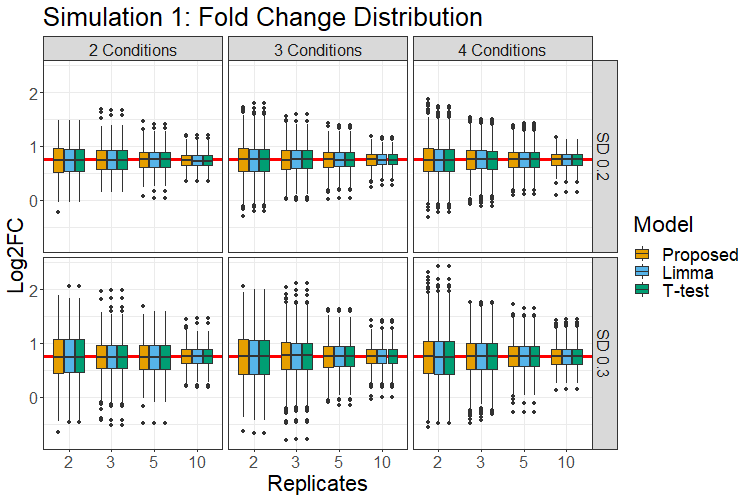
\includegraphics[width=.445\textwidth]{sim_new/sim1_FC_boxplot}
	&
	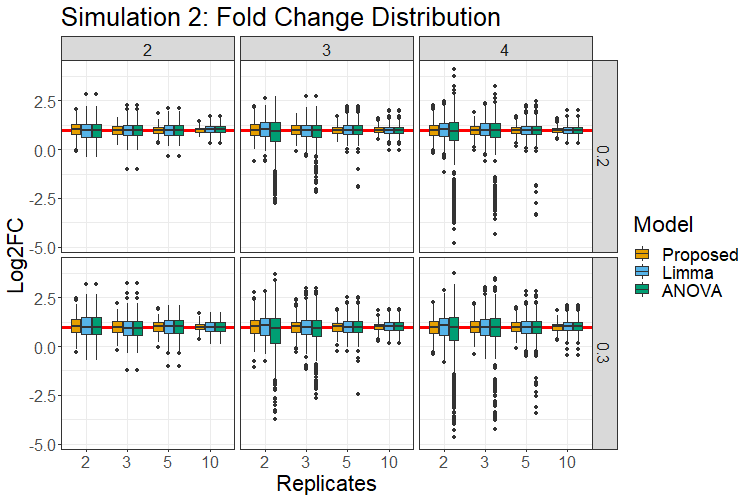
\includegraphics[width=.56\textwidth]{sim_new/sim3_FC_boxplot}\\
	(a)&(b)
\end{tabular}
\caption{\todo{In (b) could you indicate in panel labels that we are still talking about conditions and SD?}Simulated Datasets 1 and 2 : fold change distributions. (a) In Simulated Dataset 1 all considered methods correctly estimated the fold change between conditions, with a median fold change estimation of 1. The distributions around the median were also consistent across all methods. (b) In Simulated Dataset 2 all methods correctly estimated the fold change with a median log change of 1. $MSstatsPTM$ in this simulation had a  tighter distribution around the median. Both $Limma$ and $ANOVA$ showed a wider range around the fold change. \todo{In is not clear from the text whether Limma and ANOVA were used with or without adjustments for unmodified proteins. Could you clarify?}}
\label{fig:fc_boxplot}
\end{figure}

%%%%%%%%%%%%%%%%%%%%%%%%%%%%%%%%%%%%%%%%%%%%%%%%%%%%%%%%%%%%%%%%
\clearpage
\subsection{Dataset 3 : SpikeIn benchmark - Ubiquitination - Label-free}
\label{sec:benchmark}

\begin{figure}[h!]
\centering
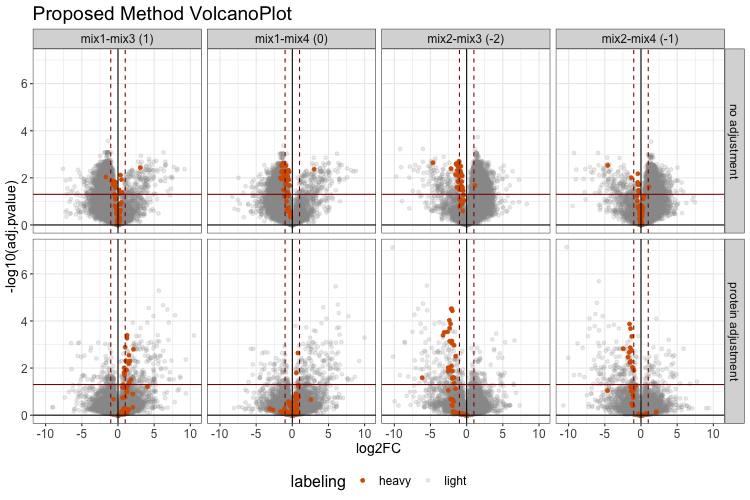
\includegraphics[width=1\textwidth]{sim_new/spike_in_msstatsptm_volcano}
\caption{\todo{Clarify that MSstats is the basic version before the adjustment, and MSstatsPTM after the adjustment} \todo{Start the caption with the name of the dataset} The modeling results of the $MSstatsPTM$ both before and after adjustment. The spike-in peptides are colored red and the background peptides are colored grey. All grey peptides are expected to not be detected as differentially abundant. The spike-in peptides (colored red) did not follow the expected log fold change before adjustment. After adjusting for changes in overall protein abundance the spike-in peptides were more in line with expectation. Additionally the background grey colored peptides showed many false positives before adjustment. After adjustment these false positives were decreased considerably. \label{fig:spike_volcano_msstats}}
\end{figure}

\begin{figure}[h!]
\centering
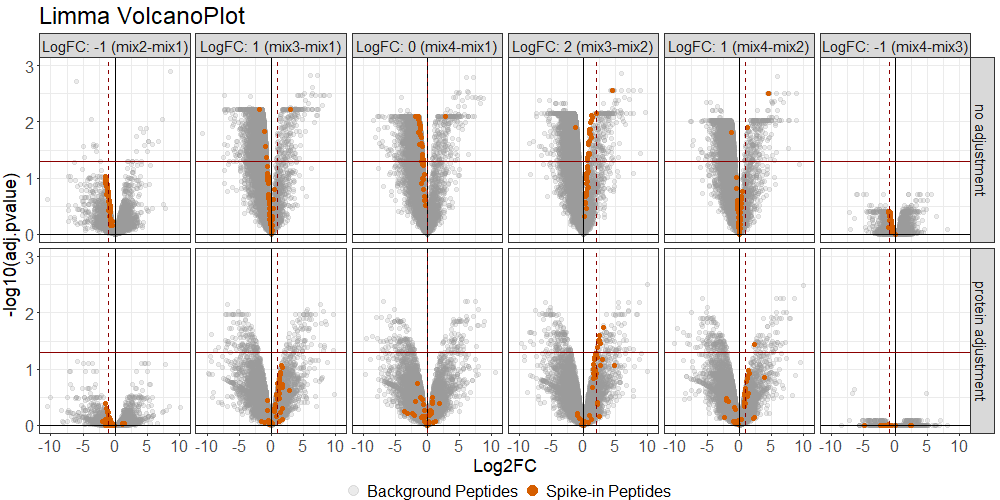
\includegraphics[width=1\textwidth]{sim_new/spike_in_limma_volcano}
\caption{\todo{Start the caption with the name of the dataset} When modeling the experiment with the $Limma$ method, the spike-in peptides again follow the expected log fold change better after adjusting for changes in protein level. However, while the fold change was more accurate, the majority of spike-in peptides were not detected as differentially abundant. There were more false positive differentially abundant PTM before than after adjustment. \label{fig:spike_volcano_limma}}
\end{figure}

\begin{figure}[h!]
\centering
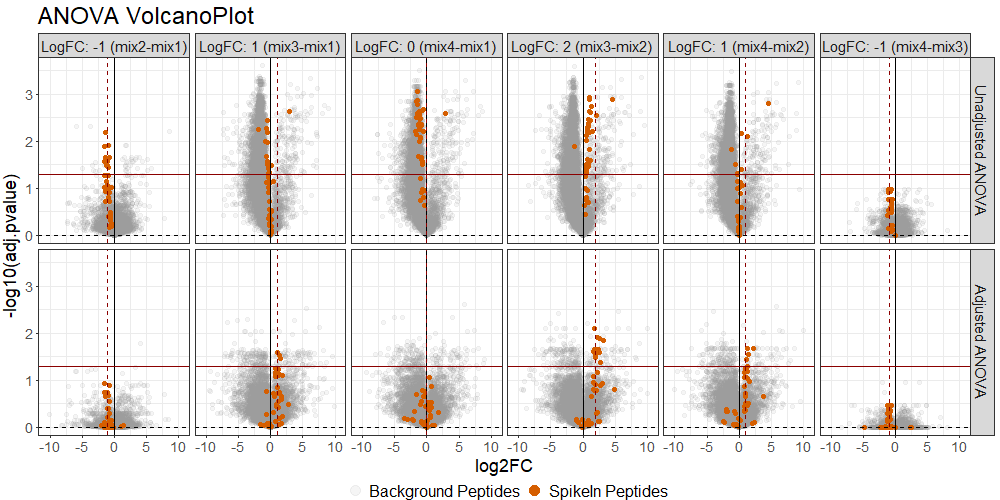
\includegraphics[width=1\textwidth]{sim_new/spike_in_anova_volcano}
\caption{\todo{Start the caption with the name of the dataset} Using $ANOVA$ the fold change of the spike-in peptides was much closer to expectation after adjusting for global protein abundance. The log FC estimation was the same as $Limma$, however the p-values were different. In this particular case we detect a few more true positives using $ANOVA$ compared to $Limma$.\label{fig:spike_volcano_ttest}}
\end{figure}

%%%%%%%%%%%%%%%%%%%%%%%%%%%%%%%%%%%%%%%%%%%%%%%%%%%%%%%%%%%%%%%%
\clearpage
\subsection{Dataset 4 : Human - Ubiquitination - 1mix-TMT}
\label{sec:ipah}

The experiment had a simple group comparison design, shown in Table~\ref{table:ipah_design}.

\begin{table}[h!]
\centering
\begin{tabular}{| c | c | c |}
\hline
 Condition & BioReplicate & Channel \\ [0.5ex]
 \hline\hline
 Dox1hr & Dox1hr\_1 & 127C\\
 \hline
 Dox2hr & Dox2hr\_1 & 128N\\
\hline
 Dox2hr & Dox2hr\_2 & 130C\\
\hline
 Dox4hr & Dox4hr\_1 & 128C\\
\hline
 Dox4hr & Dox4hr\_2 & 131C\\
\hline
 Dox6hr & Dox6hr\_1 & 129N\\
\hline
 Dox6hr & Dox6hr\_2 & 131N\\
\hline
 NoDox0hr & NoDox0hr\_1 & 126C\\
\hline
 NoDox0hr & NoDox0hr\_2 & 129C\\
\hline
 NoDox6hr & NoDox6hr\_1 & 127N\\
\hline
 NoDox6hr & NoDox6hr\_2 & 130N\\
\hline
\end{tabular}
\caption{The experimental design of Dataset 4}
\label{table:ipah_design}
\end{table}
The following model was fit separately for ubiquitinated peptides and for unmodified protein 
\begin{eqnarray*}
& Y_{mij} = \mu_i + \epsilon_{mij},\ \sum_{i=1}^I{\mu_i} = 0 ,\ \epsilon_{mij} ~ \sim N(0, \sigma^2) &
\end{eqnarray*}
\begin{figure}[h!]
 \centering
	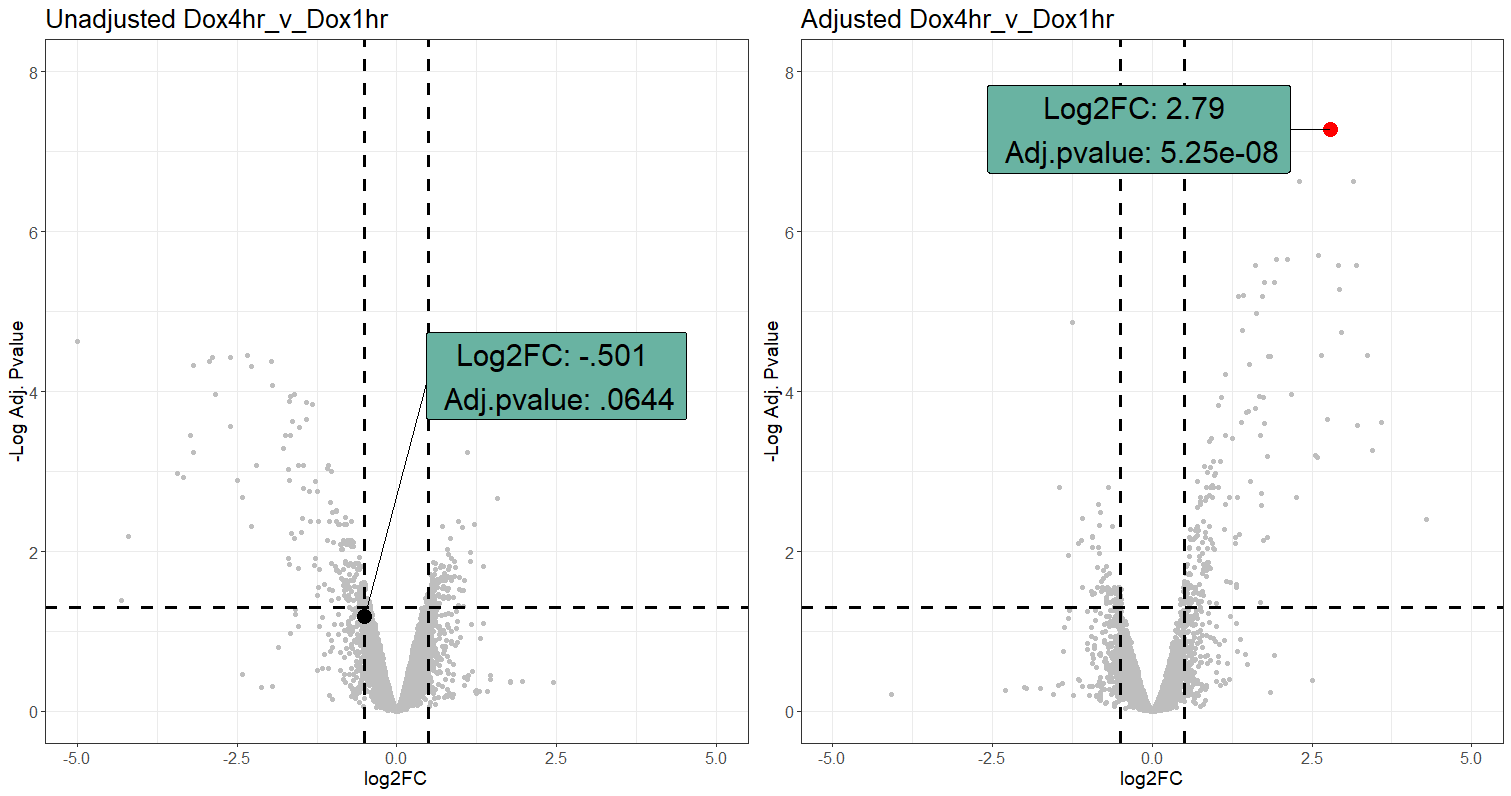
\includegraphics[width=.8\textwidth]{sim_new/IpaH_volcano_plot}
	\caption{\todo{Could you separate the panels, and add labels (a) and (b) in the subfigures. (Could you use tabular as I did everywhere?) The title of the second panel is cut off. It is not clear which method is used - is it MSstats and MSstatsPTM?} \todo{Start the caption with the name of the dataset} Volcano plots of Dox4hr vs Dox1hr both before and after protein adjustment, \todo{with $MSstatsPTM$}. The $GSDMD\_HUMAN|P57764\_K62$ modification is highlighted. (a) Before adjustment the modification had a small fold change and was not detected as differentially abundant. (b) After adjustment the fold change was much larger, and the modification was detected as differentially abundant. In this case \todo{$MSstatsPTM$?} allowed us to identify a differential modified peptide that could have otherwise been missed.}
\label{fig:ipah_figures}
\end{figure}

\clearpage
\subsection{Dataset 5 : Mouse - Phosphorylation - 2mix-TMT}
\label{sec:shigella}

The experiment had a group comparison design, and the data were acquired in two mixtures, as shown in Table~\ref{table:shigella_design}.

\begin{table}[h!]
\centering
\begin{tabular}{|c | c c | c c | c|}
\hline
 & \multicolumn{2}{c}{Mixture 1} & \multicolumn{2}{c}{Mixture 2} & Condition \\ [0.5ex]
 \hline\hline
 Uninfected & 128C & & 128C & 131C & \\
 \hline
Early (1 Hour) & 126C & 129C & 126C & 129C & WT \\
\hline
Late (3 Hour) & 127C & 130C & 127C & 130C & \\
\hline
Uninfected & 129N & 131C & 129N & & \\
\hline
Early (1 Hour) & 127N & 130N & 127N & 130N & KO \\
\hline
Late (3 Hour) & 128N & 131N & 128N & 131N & \\
\hline
\end{tabular}
\caption{The experimental design of Dataset 5}
\label{table:shigella_design}
\end{table}
The following model was fit separately for phosphorylated peptides and for unmodified protein 
\begin{eqnarray*}
& Y_{mij} = \mu_i + Mixture_m + \epsilon_{mij},\ Mixture_m ~ \sim N(0, \sigma^2_M) ,\  \sum_{i=1}^I{\mu_i} = 0 ,\ \epsilon_{mij} ~ \sim N(0, \sigma^2)&
\end{eqnarray*}

\begin{figure}[h!]
\centering
	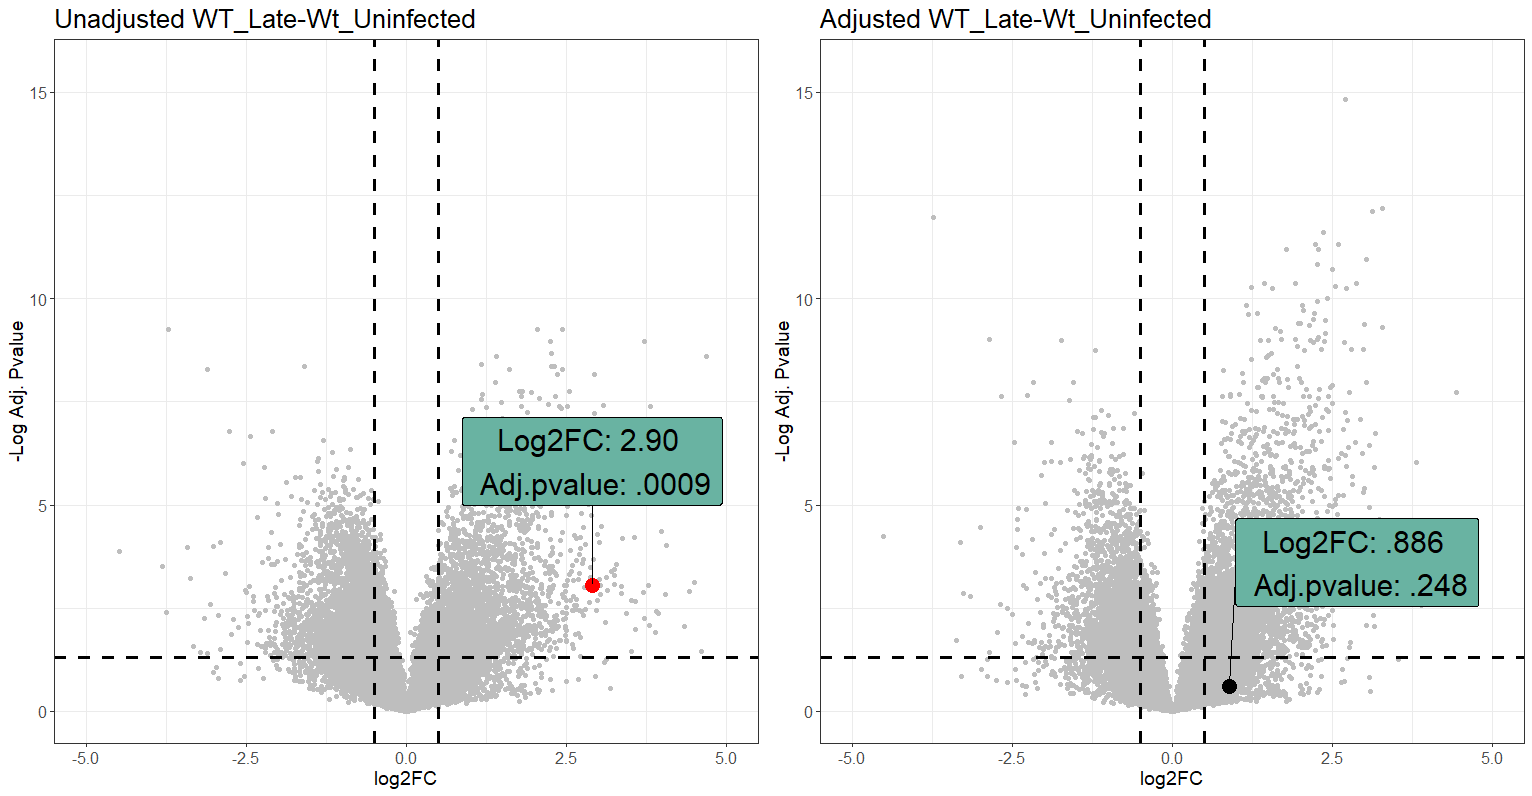
\includegraphics[width=.8\textwidth]{sim_new/No_Difference_Shigella_Volcano}
	\caption{\todo{Start the caption with the name of the dataset} \todo{Separate the labels and add labels (a) and (b) for the subpanels.  (Could you use tabular as I did everywhere?)}Volcano plots of WT\_Late vs WT\_Uninfect both before and after protein adjustment \todo{with $MSstatsPTM$}. The $TTP\_MOUSE|P22893\_S178$ modification is highlighted. (a) Before adjustment the modification had a large fold change and a small p-value. (b) After adjustment the fold change was much smaller and the modification was not detected as differentially abundant.}
\label{fig:No_Diff_Shigella_PTM}
\end{figure}

\begin{figure}[h!]
\centering
 \begin{tabular}{c}
	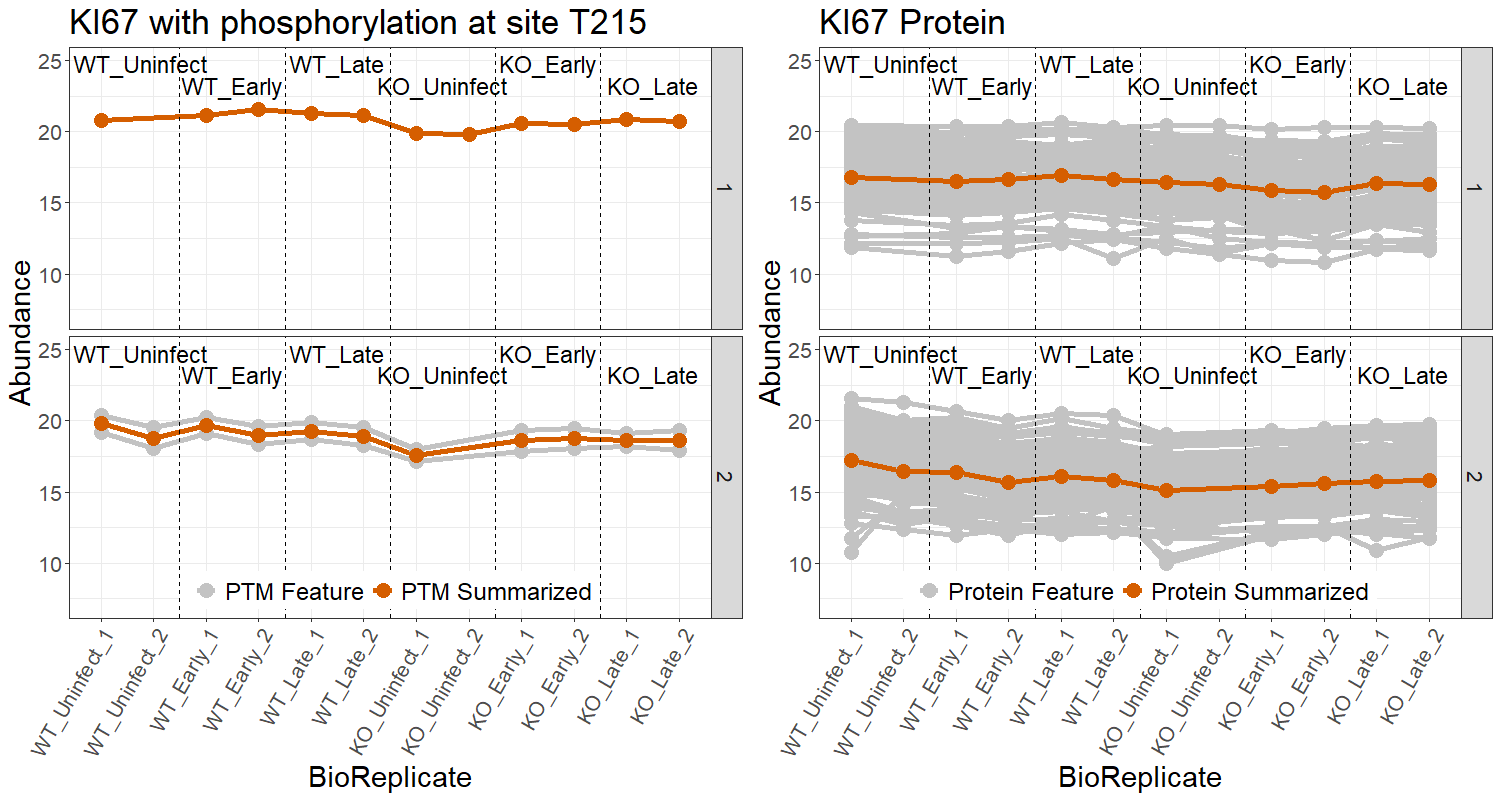
\includegraphics[width=.9\textwidth]{sim_new/Difference_Shigella_Profile_Plot}\\
	(a)\\
	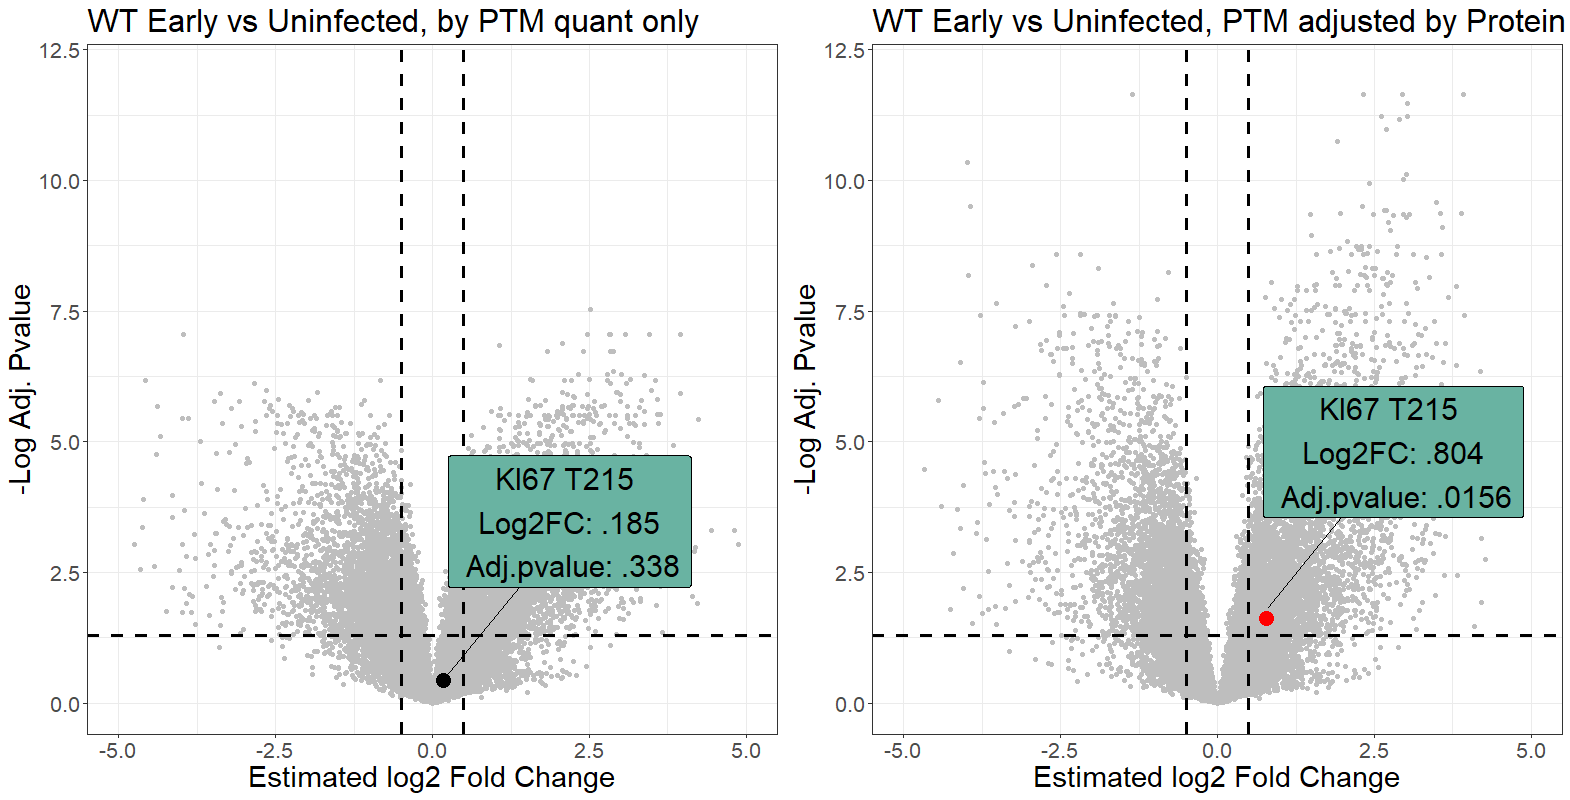
\includegraphics[width=.8\textwidth]{sim_new/Difference_Shigella_Volcano}\\
	(b)
 \end{tabular}
 \caption{\todo{Start the caption with the name of the dataset} Protein $KI67\_MOUSE|E9PVX6$ with the modification at site $T215$. (a) The modification and global protein appeared to show small or no difference between conditions when considered separately. However after adjusting for change in global protein abundance, the modification was statistically significant. Additionally, this profile plot showed the large difference in available features between modified peptides and global proteins. (b) The volcano plot of the WT\_Uninfect and WT\_Early comparison showed the specifics of the adjustment \todo{with $MSstatsPTM$}. The profile of the modified peptides appeared to be flat, with a log fold change of $.185$, while the global profiling showed a small negative fold change of $-.619$. Since both exhibit small changes in opposite directions, their combination produced a log$_2$-fold change of $.804$ and adjusted p-value of $.0156$.}
\label{fig:Diff_Shigella_PTM}
\end{figure}

\clearpage

\subsection{Dataset 6 : Human - Ubiquitination - Label-free no global profiling run}
\label{sec:usp30}

An example profile plot for this experiment can be seen in  Figure \ref{fig:USP30_profile_plot}.

\begin{figure}[h!]
\centering
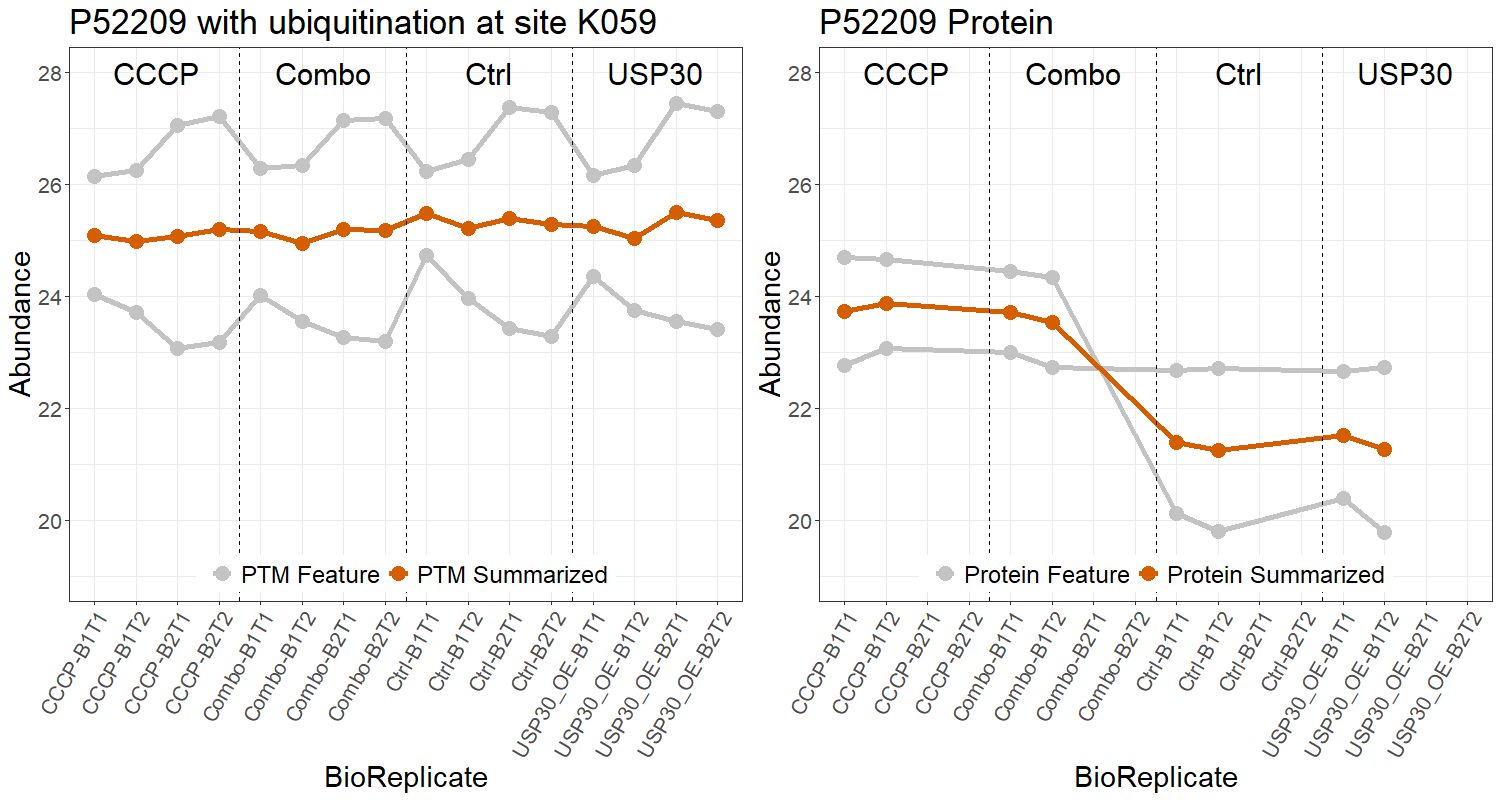
\includegraphics[width=\textwidth]{sim_new/USP30_profile_plot}
\caption{\todo{Start the caption with the name of the dataset} Protein $P52209$ with the modification of the protein at site $K059$. The modification appeared generally unchanged between all conditions, whereas the global profiling run showed that the CCCP and Combo conditions had a higher relative abundance compared to the Control and USP30\_OE. This indicated that the modification had in fact an effect when comparing CCCP and Combo to Control and USP30\_OE. However it was not entirely clear as one unmodified peptide feature appeared to be changed, while the other did not. This uncertainty was another result of not acquiring data from a separate global profiling run. A separate global profiling run would have likely resulted in more and better quality unmodified features for that protein. }
\label{fig:USP30_profile_plot}
\end{figure}


%%%%%%%%%%%%%%%%%%%%%%%%%%%%%%%%%%%%%%%%%%%%%%%%%%%%%%%%%%%%%%%%
\clearpage

\printbibliography 

\end{document} 

